\documentclass[
	conference,	% Conference-style paper, as opposed to journal-style
	%a4paper,	% Print on A4 paper (but still typeset for US letter)
]{IEEEtran}

%% Input and output encodings
\usepackage[utf8]{inputenc}	% Input: UTF-8 input text encoding
\usepackage[T1]{fontenc}	% Output: T1 font encoding

%% Math and symbols
\usepackage{amsmath}	% AMS Math: additional math typesetting
\usepackage{amsfonts}	% AMS Fonts: additional fonts for math
\usepackage{textcomp}	% Text Companion Fonts: additional symbols in text mode

%% Color

% xcolor - Provide color functionality and color names
\usepackage[
	x11names,	% See https://en.wikipedia.org/wiki/X11_color_names
	svgnames,	% See https://en.m.wikipedia.org/wiki/Web_colors
]{xcolor}

%% Figures and graphics
\usepackage{graphicx}	% Basic graphics inclusion and transform capability
\usepackage{stfloats}	% More control over spacing in floats

% subfig - Figures within figures, e.g. "Figure 3b shows..."
\usepackage[
	caption=false,
	font=normalsize,
	labelfont=sf,
	textfont=sf
]{subfig}

%% Tables
\usepackage{array}	% Extended 'array' and 'tabular' environments
\usepackage{booktabs}	% Nicer tables and more line commands (e.g. \midrule)
\usepackage{threeparttable}	% Tables with their own footnotes

%% Algorithm pseudocode
%
% See https://tex.stackexchange.com/a/230789/229926 for a nice summary of the
% different algorithm packages available.
\usepackage[noend]{algpseudocode}	% Typesetting of algorithms in pseudocode

%% Code listings
\usepackage{listings}
\lstset{
	numbers=left,		% Show line numbers, on left
	frame=none,		% Do not put a frame around the listing
	xleftmargin=2em,	% Add some extra margin on the left
}

%% A style for listings that adds color to the highlighting
\definecolor{codegreen}{rgb}{0,0.6,0}
\definecolor{codegray}{rgb}{0.5,0.5,0.5}
\definecolor{codepurple}{rgb}{0.58,0,0.82}
\definecolor{codeorange}{rgb}{0.9,0.45,0.3}
\definecolor{backcolour}{rgb}{0.95,0.95,0.92}
\lstdefinestyle{colorlisting}{
	basicstyle=\small,
	identifierstyle=\texttt,
	commentstyle=\color{codegreen},
	keywordstyle=\color{blue},
	numberstyle=\tiny\color{codegray},
	stringstyle=\color{codeorange},
	showstringspaces=false, % Do not mark in-string spaces with underscores
}

\lstset{style=colorlisting}	% Set default style
% Note that the identifierstyle from this default style will be used for all
% \lstinline usages in the text.


%% Quotes
\usepackage{csquotes}		% Context Sensitive Quotes
\MakeOuterQuote{"}		% Automatically curl double quotes
\usepackage{epigraph}		% Typeset quotes used for flavor

%% Bibliography
%\usepackage[style=ieee]{biblatex}
%\addbibresource{references.bib}

%% Links and cross-references

\usepackage{url}	% Basic URL typesetting

% hyperref - Clickable hyperlinks
%
% Note that 'hyperref' prefers to be loaded after most other packages. This is
% because hyperref redefines and enhances so many LaTeX commands that including
% some packages after it can undo or break the enhancements it has made. Only
% hyperref-aware packages should be loaded after hyperref.
%
% The hyperref manual §11.1 "Package Compatibility" has detailed notes on
% interactions with other packages.
\usepackage{hyperref}
\hypersetup{
	colorlinks=true,	% Mark links by changing text color
	linkcolor=Maroon,
	filecolor=Maroon,
	citecolor=Maroon,
	urlcolor=DarkBlue,
}

% Names used with hyperref's \autoref command
\renewcommand{\sectionautorefname}{Section}
\renewcommand{\subsectionautorefname}{Subsection}
\renewcommand{\subsubsectionautorefname}{Subsection}
\renewcommand{\appendixautorefname}{Appendix}
\newcommand{\algorithmautorefname}{Algorithm}

%% Reproducible PDF build
%
% PDF builds tend to be non-reproducible because PDF metadata includes a lot of
% local information, such as the build date and the full file path. The
% pdfprivacy package is an easy way to strip this information and get
% a reproducible build.
%
% - pdfprivacy package: https://www.ctan.org/pkg/pdfprivacy
% - Discussion on reproducible builds: https://tex.stackexchange.com/a/313605
%
\usepackage[nopdftrailerid=true]{pdfprivacy}

%% Specific hyphenation rules for words in this document
\hyphenation{op-tical net-works semi-conduc-tor IEEE-Xplore}

%% Custom structural macros
\newcommand{\newterm}[1]{\textit{#1}}
\newcommand{\booktitle}[1]{\textit{#1}}
\newcommand{\papertitle}[1]{\enquote{#1}}
\newcommand{\TeXnician}{\TeX\-nician}
\newcommand{\TeXnicians}{\TeX\-nicians}

%% Special Unicode characters

% ế LATIN SMALL LETTER E WITH CIRCUMFLEX AND ACUTE
%
% This accented 'e' appears in the name of the author of pdfTeX, Hàn Thế Thành.
% This is how he himself codes it in the pdfTeX manual.
% https://tug.org/svn/pdftex/branches/stable/doc/manual/pdftex-t.tex?revision=837&view=markup#l119
\DeclareUnicodeCharacter{1EBF}{\^e\llap{\raise 0.5ex\hbox{\'{}}}} % ế LATIN SMALL LETTER E WITH CIRCUMFLEX AND ACUTE


%% Title and author metadata

\title{{\LaTeX} Report Template in IEEE Style}

\author{
	\IEEEauthorblockN{Mike Murphy}
	\IEEEauthorblockA{
		\textit{Department of Computer Science } \\
		\textit{UiT The Arctic University of Norway}\\
		Tromsø, Norway \\
		michael.j.murphy@uit.no
	}
	\and
	\IEEEauthorblockN{Øyvind Nohr}
	\IEEEauthorblockA{
		\textit{Department of Computer Science } \\
		\textit{UiT The Arctic University of Norway}\\
		Tromsø, Norway \\
		oyvind.a.nohr@uit.no
		%userName@github
	}
}

%% Actual document

\begin{document}

\maketitle

\begin{abstract}
	This document is both an example of and a tutorial for using {\LaTeX}
	and the IEEE {\LaTeX} template to write a technical report.
	It follows a structure that can work well for systems research in
	computer science
	and
	its content is an introduction to {\LaTeX}.
	Students can use this as a template for their reports
	by replacing the content and adapting the structure.
	This template is tailored to the
	Operating Systems course (INF\nobreakdash-2201)
	at UiT The Arctic University of Norway,
	but it should be useful for other courses as well.
\end{abstract}

\begin{IEEEkeywords}
	Assignment submission, {\LaTeX}, paper, template, typesetting
\end{IEEEkeywords}


\section{Introduction}\label{introduction}

% This is a comment.
% Note that LaTeX re-flows your paragraphs when rendering to PDF.
% Extra line breaks will be smoothed out.
% You can use extra line breaks for organizational purposes.
% For example,
% many authors like to put each sentence or phrase on a line,
% making it easier to reorder them by quickly cutting and pasting lines.

The introduction section should give
a brief overview of your system
and the fundamental problem it is trying to solve.
For an assignment report,
briefly restate the assignment requirements in your own words.

This example document will explain some {\TeX} and {\LaTeX} concepts along
the way as an example of a report.


\subsection{Outline}
\label{outline}

An introduction section typically ends with a compact outline of the rest of
the paper.
The \lstinline!label!
and \lstinline!ref!
commands can be used to make cross references.
%
Use \lstinline!label! set a point in the text to refer to,
then \lstinline!ref! will give the section/subsection number where the
label appears.
For example, \label{examplereflabel}%
this is Subsection~\ref{examplereflabel}.	% "I-A"
%
The \lstinline!autoref! command gives not just the number,
but also identifies the section/subsection type
For example, \label{exampleautoreflabel}%
this is \autoref{exampleautoreflabel}.		% "Subsection I-A"

The rest of this report is organized as follows.
\autoref{background} outlines concepts and background information relevant to the project.
\autoref{relatedwork} describes related work.
\autoref{description} describes our solution.
\autoref{evaluation} describes our methodology for evaluating our solution.
\autoref{results} gives the results of our evaluation.
\autoref{discussion} discusses the results.
\autoref{futurework} describes known bugs and future plans.
And finally, \autoref{conclusion} is the conclusion.


\section{Background}
\label{background}

The background section should give
a brief review of concepts necessary to understand your solution.
In the case of Project 2 in this course, this would include concepts like
processes, threads, context switching, scheduling, user space vs kernel
space, and system calls.
In the case of this tutorial,
we will provide background on typesetting and on writing styles.


\subsection{Typesetting, {\TeX}, and {\LaTeX}}

\epigraph{{\LaTeX} is a great way to program about writing while you're
procrastinating on writing about programming.}{Mike Murphy}

Typesetting is the art of arranging text on a page for printing.
Typesetting is often judged by how well a column of text lines up at its
left and right edges,
and by how uniform the greyness of the page appears.
This involves carefully placing line breaks
and then adjusting the spacing between words
to achieve the most eye-pleasing result.
{\TeX} is a typesetting engine with a sophisticated algorithm
to do just that~\cite{Knuth1986Texbook}.
For each paragraph, it tries several different arrangements, scores them,
and chooses the one with the least overall "badness" score.

{\LaTeX} is a comprehensive set of {\TeX} macros
that make {\TeX} easier to use~\cite{Lamport1994LatexBook}.
{\LaTeX} provides infrastructure to separate a document's text and structure
from its presentation,
much like Cascading Style Sheets (CSS) later did for HTML.
It also provides infrastructure for gathering macros into modular
\newterm{packages}.
These days it is relatively rare to use plain {\TeX} without {\LaTeX}.
Plain {\TeX} is probably best left to the hard-core
\newterm{\TeXnicians}~\cite{Knuth1986Texbook}.\footnotemark

\footnotetext{A summary of relevant passages on \newterm{\TeXnician}
	terminology is available at
	\url{https://tex.stackexchange.com/a/474039/229926}}


\subsection{First Person vs. Objective Writing Styles}
\label{firstpersonvsobjective}

Some teachers are dogmatic about avoiding first-person pronouns ("I" and "we")
in reports.
The result is an \newterm{objective} tone that can sound more professional.

\begin{description}[\IEEEsetlabelwidth{First-person}]
	\item[First-person]
		"We considered several strategies for implementing the
		scheduler."
	\item[Objective]
		"For implementing the operating system scheduler, several
		strategies were considered."
\end{description}

We are not dogmatic about this.
Maintaining an objective style sometimes requires awkward phrasing or
over-reliance on passive voice.
A first-person style can often feel more natural both to write and to read.


\section{Related Work}
\label{relatedwork}

The related work section is
a compact review of other work in your project's specific subfield.
This is where you cite most of the things that you read while researching
your project. What other projects inspired yours? What are you building on?
What are you competing with?
%
A well-written Background section and Related Works section will combine to
form a crash course in the state of the art of the topic at the time the paper
was written.

In this course you will not be doing a great deal of research,
but if you, say, read up on how Linux does scheduling before you
implemented your own scheduler, this the place to write about that.

For typesetting,
Thành's,
\booktitle{Micro-typographic extensions to the
	{\TeX} typesetting system}~\cite{Thanh2000Microtypography}
gives a concise history of typesetting and explores the use of subtle
techniques to enhance the appearance of text on the page.

Lamport's original {\LaTeX} book~\cite{Lamport1994LatexBook}
is the definitive guide to {\LaTeX},
but there are also many resources available online.
%
Overleaf, an online {\LaTeX} collaboration platform,
has a wealth of documentation, including a quick tutorial:
\papertitle{Learn {\LaTeX} in 30 minutes}~\cite{OverleafTutorial30Minutes}.
%
\booktitle{The Not So Short Introduction
	to {\LaTeX2e}}~\cite{LatexTutorialNotSoShort}
is a longer tutorial (139 minutes, according to the book's subtitle).
%
The {\LaTeX} Wikibook~\cite{LatexWikibook}
is a comprehensive but accessible crowdsourced guide.
%
And
\booktitle{{\LaTeX2e}: An Unofficial Reference Manual}~\cite{latex2eReference}
is a detailed reference for {\LaTeX}'s many commands.

The IEEE {\LaTeX} template
comes packaged with two helpful example documents.\footnotemark
\footnote{The IEEE {\LaTeX} template should be bundled
	with the source of this document.
	It is also available for download at
	\url{https://www.ieee.org/conferences/publishing/templates.html}}
%
\papertitle{How to Use the IEEEtran {\LaTeX}
	Class}~\cite{Shell2015HowToIEEtran}
explains the many options and commands that the template provides.
%
And the example document,
named \lstinline{conference_101719.pdf} or similar,
is filled in with advice on typographic and grammatical details,
such as avoiding math and citations in the abstract,
keeping units of measurement consistent,
and reminders about English words that are easy to mix up.

Those who wish to learn the inner workings of {\TeX}
and become {\TeXnicians}
must read Knuth's original \booktitle{\TeX book}~\cite{Knuth1986Texbook}.
%
There are also several books available online,
including
\booktitle{{\TeX} for the Impatient}~\cite{TexForTheImpatient},
\booktitle{{\TeX} by Topic}~\cite{Eijkhout1992TexByTopic},
and a separate {\TeX} Wikibook~\cite{TexWikibook}.

For advice on actually \emph{writing} a report,
the short paper
\papertitle{The ABC of academic writing: non-native speakers'
	perspective}~\cite{Nakagawa2024ABC}
offers some concise writing advice that is especially geared towards
those who are not native English speakers.
To go deeper on the subject of \emph{technical} writing,
useful books include
Alley's \booktitle{The Craft of Scientific Writing}~\cite{AlleyMichael2018TCoS}
and
Young's \booktitle{The Technical Writer's
	Handbook}~\cite{Young2002TechnicalWritersHandbook}.


\section{System Description}
\label{description}

Actually describe the system you built.
We like to describe a system from the top down
at four different layers of abstraction:
\newterm{idea,}
\newterm{architecture,}
\newterm{design,}
and
\newterm{implementation.}


\subsection{Idea}
\label{idea}

Start with an extremely high-level "elevator pitch" for your system.
What is the main idea that motivates it and sets it apart from similar
existing systems?

Since the assignments have relatively fixed requirements,
you will probably not have a lot to write here.
You can omit this subsection or you can restate the requirements,
the problem you are trying to solve.

\subsection{Architecture}
\label{architecture}

\begin{figure}[t]
	% This is an example figure.
	% The '[t]' after the opening tells LaTeX that it should
	% place the figure at the top of a column.
	% The other options are 'h' for "here", 'b' for "bottom,
	% and 'p' for a separate page.
	% You can place multiple letters in the brackets
	% to give LaTeX multiple placement options.
	% It will choose what it thinks is the best one
	% according to internal heuristics.
	% In a scientific paper, top ('[t]') is the most common option.
	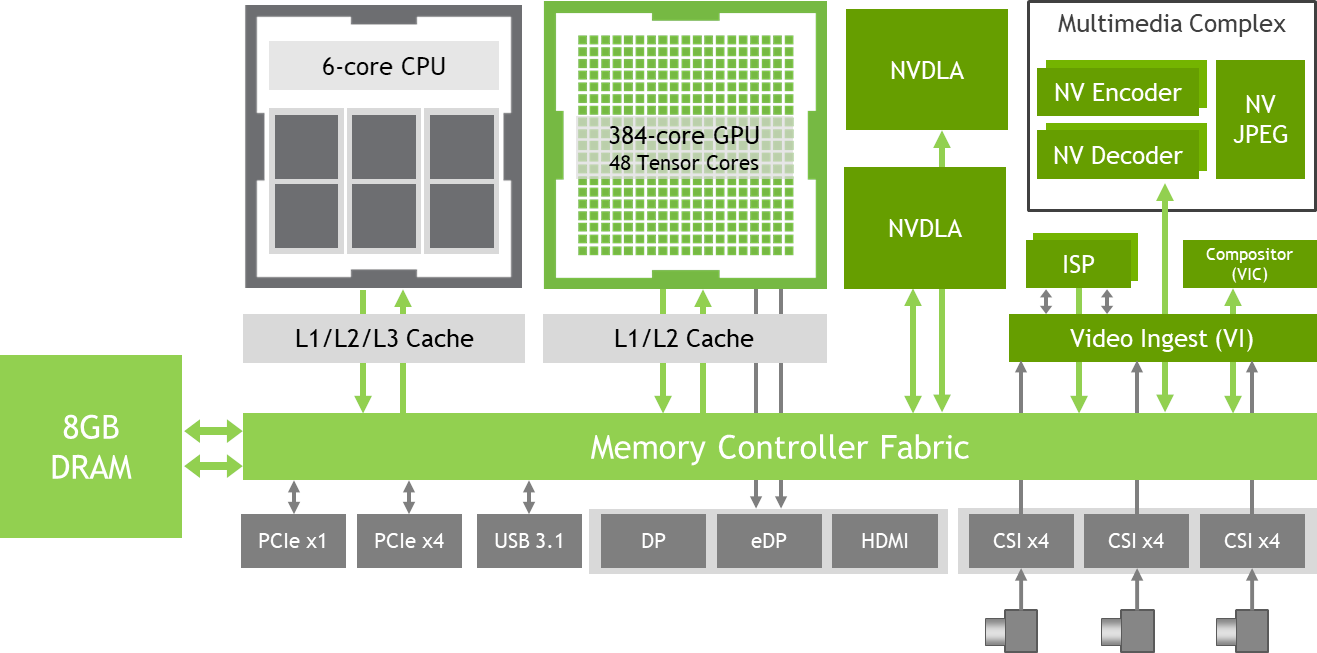
\includegraphics[width=\columnwidth]{figures/jetson_nx.png}
	\caption{Block diagram of the Nvidia Jetson Xavier NX module}
	\label{jetsonnx_blockdiagram}
	% Note the order of declarations: image, then caption, then label.
	% By convention, captions for images usually go below the image.
	% For other floats that contain mostly text
	% (e.g. tables, algorithms, and code listings),
	% the caption acts more like a title,
	% and is thus more commonly placed above.
	%
	% Either way, the \label must come after (or inside) the \caption.
	% Labels stick to the most recent previous numbered text entity,
	% and for floats it is the \caption within the float that is numbered,
	% not the float environment itself.
\end{figure}

Then begin describing the system itself, still at a very high level.
What are its major components and how do they connect?
What are the most essential factors that shaped the highest-level
structure of your system?

This is a good place for a high-level block diagram.
\autoref{jetsonnx_blockdiagram} shows a block diagram of the
Nvidia Jetson Xavier edge computing AI module.
Figures are part of a class of
{\LaTeX} document elements called \newterm{floats}
because they float to other positions on the page.
In a scientific paper, floats tend to work best at the top of a column.


\subsection{Design}
\label{design}

\begin{figure}[t]
	% Note that the IEEE template prefers you use the figure environment
	% to float algorithms, NOT the algorithm environment.
	% See How to Use the IEEEtran LaTeX Class, Section X-B.
	\begin{algorithmic}[1]
		\Procedure{OnFloatDeclaration}{}
			\If{specifier contains '!'}
				\State placement restrictions are ignored
			\Else
				\State placement restrictions are enforced
			\EndIf
			\If{specifier contains 'h'}
				\State try to place float \emph{here} in text
			\EndIf
			\If{not already placed and specifier contains 't'}
				\State try to place float in top area
			\EndIf
			\If{not already placed and specifier contains 'b'}
				\State try to place float in bottom area
			\EndIf
			\If{not already placed}
				\State add float to the holding queue
			\EndIf
		\EndProcedure
		\Procedure{OnFinishColumn}{}
			\If{holding queue not empty}
				\If{any floats in queue have 'p' specifier}
					\State use them to create a float page
				\EndIf
			\EndIf
			\If{holding queue still not empty}
				\State{attempt to place 't' and 'b' floats in next column}
			\EndIf
		\EndProcedure
	\end{algorithmic}
	\caption{Abridged pseudocode for the {\LaTeX} float placement
		algorithm~\cite{Mittelbach2014FloatAlgorithm}}
	\label{floatplacement}
\end{figure}

Now go a little deeper, but not too detailed.
What are the smaller components inside the major ones?
What factors shaped your design decisions as you fleshed out the
architecture?
Give pseudocode for important algorithms or protocols that make your
system unique.
At this level, someone reading your report should be able to write
a similar system in a different programming language or for a different
architecture.

{\LaTeX} has a sophisticated algorithm
for placing floats~\cite{Mittelbach2014FloatAlgorithm}.
Simplified pseudocode for this algorithm is shown in \autoref{floatplacement}.
When {\LaTeX} encounters a float declaration in the source,
it tries to place it at one of the locations specified by the declaration.
The top priority is "here" placement ('h'),
followed by top of the current column ('t'),
and finally bottom of the current column ('b').
If it cannot place the current float in the current column,
it places the float in a holding queue.
Then,
when it finishes a column,
it attempts to empty the holding queue.
First it attempts to create a \newterm{float page} containing
all floats in the queue that had the "page" placement specifier ('p').
Then it attempts to place the next top and bottom floats
from the queue into the next column.

Note that the {\TeX} engine works one column at a time,
and it cannot backtrack.
Once a column has been set, {\TeX} flushes its output, reclaims that memory,
and moves on to the next column.
Therefore,
depending on how your columns flow,
you may have to declare a figure far ahead of the section that references it
in order to have it appear in the desired column.
Even then, editing your text may cause columns to reflow,
which may cause floats to end up in wildly different places.
That is why the common advice is to not worry about figure placement until the
very end of the editing process,
after you have stopped changing the actual text.


\subsection{Implementation}
\label{implementation}

\begin{figure}
\begin{lstlisting}[language=C]
/* Simple copy from src to dest */
char *strcpy(char *restrict dest,
		const char *restrict src)
{
    char *destorig = dest;
    for (;; dest++, src++) {
	char copiedchar = *dest = *src;
	if (!copiedchar) break;
    }
    return destorig;
}
\end{lstlisting}
\caption{An implementation of \lstinline{strcpy} in C}
\label{strcpy}
\end{figure}

Finally, describe implementation details such as programming language
used and target hardware.

This {\LaTeX} document can be rendered with a standard
{\TeX} Live distribution\footnote{\url{https://www.tug.org/texlive/}}
plus the IEEE {\LaTeX} template.%
\footnote{\url{https://www.ieee.org/conferences/publishing/templates.html}}
The build is controlled by GNU Make,%
\footnote{\url{https://www.gnu.org/software/make/}}
with help from the latexmk script.%
\footnote{\url{https://www.ctan.org/pkg/latexmk}}

Actual code listings will typically be too low-level to include in your report.
But if you do need to list code, you can use the \lstinline!listings! package.
An example code listing is shown in \autoref{strcpy}.


\subsection{Image Formats}
\label{imageformats}

Images like diagrams, plots, and logos
look best when the source image is in a
\newterm{vector-based} image format,
where shapes and curves are described geometrically,
rather than a \newterm{rasterized} format,
where the image is stored as a grid of pixels.
Raster formats like JPEG and PNG will look pixelated if one zooms in on them,
but vector formats can be re-rendered crisp and smooth at any resolution.
When drawing diagrams and generating plots from data,
be sure to export them to a vector-based format like PDF or SVG.
The default {\LaTeX} program,
\lstinline!pdflatex!
can include other PDFs natively.
SVG support can be enabled by using the
\lstinline!svg! package,\footnote{\url{https://www.ctan.org/pkg/svg}}
but be aware that the \lstinline!svg! package
enables SVG support by quietly converting them to PDFs during processing.
This requires that you have
Inkscape\footnote{\url{https://inkscape.org/}}
installed to perform the conversion.

% TODO: Discuss diagram drawing tools like Inkscape, Graphviz, and TikZ.

\section{Evaluation}
\label{evaluation}

Describe the methods used to evaluate the system.
Define the metrics used to measure performance,
and the procedures used to gather metrics.
Include details like the specs of the hardware that ran the experiments.
Do not include results yet.
Those go in the next section.


\section{Results}
\label{results}

\begin{table}[t]
	\caption{Precision results of classifiers for different feature sets}
	\label{classifierprecisionresults}
	\begin{tabular*}{\linewidth}{@{\extracolsep{\fill}} l cc cc cc @{}}
		\toprule & \multicolumn{6}{c}{Precision} \\
		\cmidrule{2-7}
		Classifier          & (1)\tnote{a} & (2)\tnote{b}  & (3)\tnote{c}  & (1\&2)\tnote{d} & (1\&3)\tnote{e} & All\\
		\midrule
		Perceptron          & 0.78 & 0.82 & 0.24 & 0.81 & 0.77  & 0.83\\
		Decision Tree       & 0.65 & 0.79 & 0.56 & 0.75 & 0.65  & 0.73\\
		One-Class~SVM       & 0.74 & 0.72 & 0.50 & 0.80 & 0.73  & 0.85\\
		Isolation Forest    & 0.54 & 0.51 & 0.52 & 0.53 & 0.54  & 0.53\\
		\bottomrule
		\newline
	\end{tabular*}
\end{table}

Give the results of the evaluation, including data tables and plots.
Describe your results in a very concrete, quantitative way.
Just the facts.
Qualitative discussion can go in the next section.

An example data table is show in \autoref{classifierprecisionresults}.
In this experiment,
the One-Class SVM classifier had the highest over-all precision score at 0.85,
followed by Perceptron at 0.83,
Decision Tree at 0.73.
Isolation Forest had the lowest precision, with a score of 0.53.

If you plot your data,
be sure to export the plot in a vector-based format
as noted in \autoref{imageformats}.

% TODO: Include a plot. Discuss plotting tools like Matplotlib.


\section{Discussion}
\label{discussion}

Discuss your system, your experiments, and your results in a more
qualitative way.
What are the positives and negatives?
Discuss unexpected results and their implications.

Discuss alternative solutions.
What other designs did you consider?
Why did you reject them?
What are the trade-offs involved?
Show that you understand the problem
and the different ways it might be solved.
Show the thought that you put into your system.

This is also a section where you can tell more of a story about your project.
Did you first try other designs that did not work?
Were there difficult bugs that you had to work out
or other difficulties that you had to overcome?


\section{Future Work}
\label{futurework}

Discuss possible ways to improve or expand the system.
If there are known bugs that you were not able to fix,
describe them here and offer suggestions for how you would fix them
if you had more time to do so.
Similarly, if there are parts of your design that you are not satisfied with,
describe how you would change them if you had more time.


\section{Conclusion}
\label{conclusion}

Briefly restate the key points of your work and wrap up the paper.

Note that it is ok if your report does not follow this structure exactly.
Since the parameters of your assignments in this course are relatively narrow,
you may not have a lot of content for every section listed.
In that case you may shorten or combine sections,
but try to follow the spirit of the template.


% Do a column break here to get even columns on the last page
%\vfill\pagebreak
% Do a column break in the bibliography to get even columns on last page
\IEEEtriggeratref{10}


%% Bibliography
\bibliographystyle{IEEEtran}
\bibliography{IEEEabrv,references.bib}

%% Appendix
\appendices


\section{Use of Generative A.I.}

Generative artificial intelligence tools were not used in writing this report.

In this course, we do not forbid you from using generative A.I. tools
like ChatGPT,
but we do discourage their use.
We encourage you to write for yourself because it is a good exercise in
collecting your thoughts and expressing them clearly.
Good writing takes practice, and these reports are a chance to practice.

If you do use ChatGPT or other generative AI tools,
you must add a section to your report explaining what tools you used and
how you used them.
For example, if you used a ChatGPT to generate a draft that you then edited,
say that.


\section{Pro Touch: Even Columns on Last Page}

IEEE likes to have the two columns on the last page be about even length.
To accomplish this, you can add a manual column break in your text.
If the target place for the break is in normal text,
you can use the following commands:

\begin{lstlisting}[language=tex,numbers=none]
\vfill\pagebreak
\end{lstlisting}

The \lstinline!\vfill! fills the rest of the vertical space in the column
that you are ending,
so that {\LaTeX} does not try to stretch the text to fit.
And then the command to end a column is actually \lstinline!\pagebreak!
because internally columns are treated as miniature pages.

If the target place for the break is in the bibliography,
you can use a special command that IEEE provides as part of the template:

\begin{lstlisting}[language=tex,numbers=none]
\IEEEtriggeratref{10}
\end{lstlisting}

This will cause a column break before reference number ten.

\end{document}
